% Ti--Al manuscript: revised draft, 3 November 2026.
% AIP / Journal of Chemical Physics format, REVTeX 4.2.
% Switch reprint to preprint for a single-column editing copy.
\documentclass[aip,jcp,reprint,superscriptaddress,amsmath,amssymb,longbibliography,floatfix]{revtex4-2}
\usepackage[T1]{fontenc}
\usepackage[utf8]{inputenc}
\usepackage{graphicx}
\usepackage{bm}
\usepackage[colorlinks=true,linkcolor=blue,citecolor=blue,urlcolor=blue]{hyperref}
\newcommand{\rscan}{\ensuremath{r^{2}}SCAN}
\newcommand{\draftnote}[1]{\par\smallskip\noindent{\small\textbf{Draft note.} \textit{#1}}\par\smallskip}
\begin{document}
\title{Assessing exchange-correlation effects in Ti--Al alloys with fine-tuned foundation interatomic potentials}
\author{N. N. Katkov}
\affiliation{Vatolin Institute of Metallurgy of the Ural Branch of the Russian Academy of Sciences, Amundsena Street 101, Yekaterinburg 620016, Russia}
\author{E. O. Khazieva}
\affiliation{Vatolin Institute of Metallurgy of the Ural Branch of the Russian Academy of Sciences, Amundsena Street 101, Yekaterinburg 620016, Russia}
\author{R. E. Ryltsev}
\email{rrylcev@mail.ru}
\affiliation{Vatolin Institute of Metallurgy of the Ural Branch of the Russian Academy of Sciences, Amundsena Street 101, Yekaterinburg 620016, Russia}
\affiliation{Ural Federal University, 620002 Ekaterinburg, Russia}
\date{Draft -- 3 November 2026}
\begin{abstract}
Machine-learning interatomic potentials inherit the exchange-correlation approximation used to generate their reference data, but its effect on finite-temperature alloy properties remains difficult to assess systematically.
We compare Ti--Al potentials obtained by fine-tuning the DPA4-Neo foundation model on PBE, PBEsol, and \rscan{} datasets derived from a common pool of 1000 selected configurations.
Common DFT labeling and fine-tuning settings support comparisons across lattice dynamics, density, melting, liquid mixing thermodynamics, and viscosity. Matched direct-DFT and DPA4 phonon calculations distinguish discrepancies with experiment in the reference description from residual errors in the fine-tuned harmonic response.
The clearest improvement with \rscan{} is found for the melting temperature of Ti: the coexistence estimate increases from approximately 1750--1760~K for the GGA-based potentials to 1855~K, reducing the deviation from the experimental value of 1943~K from about 9--10\% to 4.5\%.
The \rscan{} model also improves the overall description of the liquid mixing enthalpy at 2000~K, although its broad minimum near $x_{\mathrm{Al}}=0.5$--0.6 is somewhat too exothermic.
These gains do not extend uniformly to other observables: PBE gives closer agreement with the liquid-density references and most of the available alloy-viscosity reference values, while harmonic phonons and pure-Ti viscosity show no uniform functional ranking.
The results identify relative phase and mixing energetics as promising areas for \rscan{}-based Ti--Al potentials and demonstrate why exchange-correlation choices must be assessed against several complementary properties.
\end{abstract}

\maketitle
\section{Introduction}
\label{sec:introduction}

Titanium aluminides combine low density with high specific strength and creep resistance at elevated temperatures, making them attractive for lightweight components in aircraft and automotive engines.\cite{Clemens2013}
The binary Ti--Al system provides the chemical basis for these alloys and contains several ordered compounds, including $\gamma$-TiAl and $\alpha_2$-Ti$_3$Al.
Their processing and performance involve both crystalline phases and the liquid state.
In particular, simulations of melting and solidification require an accurate description of phase stability, while the density, mixing thermodynamics, and viscosity of the melt provide complementary information about its behavior during processing.
Developing an atomistic description that remains reliable across compositions and phases is therefore an important problem for Ti--Al alloys.

Considerable effort has already been devoted to constructing interatomic potentials for this system.
Established approaches include the embedded-atom potentials of Zope and Mishin\cite{Zope2003} and the second-nearest-neighbor modified embedded-atom potential of Kim \textit{et al.}\cite{Kim2016}
Machine-learning interatomic potentials (MLIPs) have subsequently expanded the flexibility of the representation and the range of reference configurations that can be included in training.
Examples include the polynomial-invariant potentials of Seko for binary Ti--Al,\cite{Seko2020} the neuroevolution potential developed by Zhao \textit{et al.} for Ti--Al--Nb,\cite{Zhao2024} and the Ti--Al neuroevolution potential of Shen \textit{et al.}\cite{Shen2025}
Recent work has also examined the transferability of broadly trained potentials to Al--Ti melts, including their composition-dependent thermophysical and transport properties.\cite{Song2024,Kato2026}
These studies establish a substantial basis for atomistic modeling of Ti--Al and make the accuracy of the underlying reference description an increasingly relevant question.

The three system-specific MLIP studies cited above use density-functional theory (DFT) reference calculations with the Perdew--Burke--Ernzerhof (PBE) exchange-correlation functional.\cite{Seko2020,Zhao2024,Shen2025,Perdew1996}
Agreement with such reference data measures how accurately a potential reproduces the selected DFT approximation; agreement with experiment also depends on the physical accuracy of that approximation.
The melting temperature of elemental Ti provides a particularly clear example.
Zhao \textit{et al.} report a value of $1671\pm5$~K, compared with their experimental reference of 1941~K,\cite{Zhao2024} whereas Shen \textit{et al.} obtain 1611~K against 1943~K.\cite{Shen2025}
Both models reproduce a range of crystalline properties, yet their Ti melting temperatures are lower than experiment by approximately 14--17\%.
These discrepancies motivate an explicit examination of exchange-correlation effects.
Differences in training coverage, fitting errors, and simulation protocols must also be considered when comparing the predictions of distinct MLIPs.

Melting and liquid transport are demanding tests because they probe aspects of the potential-energy surface that are not fully characterized by equilibrium crystal properties.
The melting temperature depends on the free-energy balance between the solid and liquid, and viscosity depends on the relaxation of microscopic stress fluctuations.
Consequently, small regression errors for energies and forces do not by themselves establish quantitative accuracy for either observable.
First-principles calculations accelerated by machine-learned force fields have shown that predicted melting temperatures depend appreciably on the exchange-correlation approximation.\cite{Jinnouchi2019}
For alloy liquids, this dependence can additionally vary with composition, making a comparison over the binary composition range more informative than a test of the pure elements alone.

Our recent study of Al--Cu melts demonstrated the practical importance of this issue.\cite{Khazieva2024}
PBE-based potentials described a broad set of properties but failed to reproduce the measured composition dependence of viscosity in the Cu-rich region.
Fine-tuning on reference data calculated with PBEsol or \rscan{} substantially improved the description of thermodynamic and transport properties; the \rscan{} potential reproduced the experimentally observed viscosity maximum.
That work also showed that transfer learning can reduce the amount of reference data needed to construct potentials at a different level of electronic-structure theory.
These results motivate a corresponding assessment for Ti--Al, where the balance between crystalline and liquid properties, and its variation with composition, remains to be established for alternative functionals.

PBEsol and \rscan{} provide two distinct alternatives to PBE for this comparison.
PBEsol modifies the generalized-gradient approximation to improve the description of densely packed solids and their surfaces,\cite{Perdew2008} whereas \rscan{} is a regularized, constraint-restored meta-generalized-gradient approximation.\cite{Furness2020}
Their different constructions offer an opportunity to examine how changes in the reference electronic-structure approximation affect crystalline and liquid observables within a common MLIP framework.
Improved agreement for one property need not imply an equivalent improvement for the others, so the assessment must include several independent physical benchmarks.

Foundation interatomic models make such comparisons more accessible.
Pretraining on broad chemical and structural datasets provides representations that can be adapted to a particular system using a comparatively compact reference dataset.\cite{Batatia2025}
Transfer learning can then be used to change both the material domain and the electronic-structure level represented by the potential.\cite{Khazieva2024}
The recently introduced DPA4 architecture provides an equivariant, energy-conserving framework for this purpose.\cite{Li2026DPA4}
Its forces are obtained as derivatives of the predicted energy, and pretrained DPA4 models are available in several sizes.
Here we use DPA4-Neo as the common starting model for fine-tuning.
Using the same pretrained backbone and configuration-selection strategy provides a consistent basis for examining the effect of changing the DFT reference functional.

In this work, we develop Ti--Al MLIPs using PBE, PBEsol, and \rscan{} reference calculations and compare their predictions for crystalline and liquid states.
The reference configurations are selected from a common pool generated by foundation-model molecular dynamics and structural relaxation, and are used to fine-tune the DPA4-Neo model.
We assess lattice dynamics, temperature-dependent density, the melting temperature of Ti, and the composition dependence of liquid density and mixing enthalpy.
Liquid viscosity provides an additional comparison between the PBE- and \rscan{}-based models.
The combined benchmarks allow us to determine which improvements persist across observables and which depend on composition or phase.
The resulting assessment addresses the choice of electronic-structure reference data for Ti--Al MLIPs and the use of foundation-model fine-tuning as a practical route to that comparison.

\section{Computational methods}
\label{sec:methods}

\subsection{Configuration generation and selection}
\label{sec:configurations}

The reference database was constructed in two stages: exploration of Ti--Al configurations with a pretrained potential, followed by DFT labeling of a compact representative subset.
The medium MACE-MPA-0 foundation model was used for the exploration stage,\cite{Batatia2025} with molecular dynamics and structural optimization implemented through the Atomic Simulation Environment (ASE).\cite{Larsen2017}
The configuration pool combined liquid trajectories, configurations sampled during relaxation from liquid snapshots, and trajectories initiated from substitutional solid solutions.
The crystalline parent structures included hcp and bcc Ti, $\gamma$-TiAl, and $\alpha_2$-Ti$_3$Al.
Off-stoichiometric configurations were generated by randomly replacing atomic species on the parent lattices.
These structures were random substitutional realizations; no optimization of special quasirandom structures was performed.

The solid-solution sampling runs were carried out at 1000~K for 10~ps, whereas the liquid-generation scripts used 2000~K and included alternating MD and relaxation stages.
The exploration dynamics used a 1~fs time step and a target pressure of 1~bar.
Relaxation trajectories supplemented the finite-temperature configurations with lower-energy local environments.
MACE energies and forces were used to generate this pool; the targets for fine-tuning were subsequently obtained from DFT.
% The initially described 1 ps interval between liquid relaxation starts is
% not asserted here: archived script variants use 100 or 500 MD steps.

Representative structures were selected with ASAP\cite{Cheng2020} using smooth overlap of atomic positions (SOAP) descriptors.\cite{Bartok2013}
The SOAP expansion used a radial cutoff of 3.2~\AA, a Gaussian width of 0.4~\AA, four radial basis functions, and angular terms up to $l=3$, with Ti--Al cross-species contributions included.
Atomic descriptors were averaged over each periodic configuration.
Farthest-point sampling in this descriptor space reduced the pool to 1000 configurations.
The selected set contained 880 structures with 216 atoms, 104 with 250 atoms, and 16 with 256 atoms, and included both pure elements and alloy compositions.
% FPS is inferred from the archived ASAP command, which leaves the algorithm
% at the documented default. Record the installed ASAP version before release.

\subsection{Electronic-structure reference calculations}
\label{sec:dft}

Single-point DFT calculations were performed at the selected geometries using VASP\cite{Kresse1996} and the projector augmented-wave method.\cite{Blochl1994,Kresse1999}
Three reference descriptions were considered: PBE, PBEsol, and \rscan.
The supplied PAW datasets were Ti\_pv, with ten valence electrons, and Al, with three valence electrons.
All three reference datasets were generated with a common numerical protocol in VASP~6.3.2 using non-spin-polarized calculations, a plane-wave cutoff of 550~eV, and an electronic convergence threshold of $10^{-6}$~eV.
First-order Methfessel--Paxton smearing with a width of 0.1~eV was employed.
The calculations used the \texttt{Accurate} precision setting, automatic real-space projection, and nonspherical contributions to the PAW exchange-correlation terms.
Explicit configuration-dependent reciprocal-space grids contained 8--12 full-grid points, reduced to 4--6 points in the supplied \texttt{KPOINTS} files.
These grids excluded $\Gamma$ and were identical for a given configuration across all three functionals.
The ions and simulation cells were held fixed during labeling.

The resulting datasets supplied total energies, atomic forces, and virials for fine-tuning.
Their sizes and training/validation partitions are listed in Table~\ref{tab:datasets}.
All retained structures could be matched to the common set of 1000 selected configurations; 992 configurations were present in all three labeled datasets.
There was no configuration overlap between the training and validation subsets of an individual functional.
The partitions were constructed separately, however, and were not identical across functionals.
Accordingly, errors on these validation subsets characterize approximation of the respective DFT datasets and are not treated as errors on a shared independent test set.

\begin{table}[tb]
\caption{Numbers of configurations in the fine-tuning datasets. The selected pool contains 1000 configurations.}
\label{tab:datasets}
\begin{ruledtabular}
\begin{tabular}{lrrr}
Reference & Total & Training & Validation \\
\hline
PBE      & 999 & 850 & 149 \\
PBEsol   & 998 & 849 & 149 \\
\rscan   & 993 & 845 & 148 \\
\end{tabular}
\end{ruledtabular}
\end{table}

\subsection{Fine-tuning DPA4-Neo}
\label{sec:finetuning}

The three Ti--Al potentials were initialized from the pretrained DPA4-Neo model,\cite{Li2026DPA4} using the checkpoint \texttt{DPA4-Neo-OMat24-v20260805.pt}.
Training used the PyTorch implementation in DeePMD-kit.
All three fine-tuning runs used the same hyperparameters, with a 6.0~\AA{} cutoff, two interaction blocks, 32 channels, 16 radial functions, and maximum angular order $l_{\max}=3$.
Energy-derived forces preserve the conservative form of the potential during adaptation.

Low-rank adaptation (LoRA)\cite{Hu2021} was enabled with rank 16 and scaling parameter 16.
The training schedule comprised 50 epochs, with a cosine learning-rate decay from $10^{-4}$ to $10^{-6}$.
The warm-up occupied 0.3\% of the schedule and started at 0.2 times the initial learning rate.
Optimization used HybridMuon with a weight decay of 0.01 and gradient-norm clipping at 5.
The loss combined mean-absolute-error terms for energy, forces, and virial, with constant prefactors of 20, 20, and 5, respectively; the force-norm option was enabled.
Automatic batch sizing was set to \texttt{auto:128}.
The model parameters used single precision, with automatic mixed precision enabled for training.
Source-checkpoint and frozen-export identities are recorded by cryptographic hashes for the held-out evaluation.
% Do not interpret "auto:128" as 128 structures per batch.
% Exact loss normalization / force-norm implementation and optimizer version
% must be pinned to the installed DPA4 code before reproducing the training.

For PBE, the checkpoint at 15\,000 optimization steps (15k) was selected for the updated physical-property calculations as a compromise between training/validation accuracy and the harmonic dynamics of hcp Ti.
Its energy and force errors on the complete training and validation sets are lower than at 5k, while it gives the closest integral agreement with the archived PBE DFT phonon density of states among the five saved checkpoints.
This is a joint error-and-property criterion, not early stopping at a minimum of validation loss: later checkpoints further reduce energy error.
For the DFT-reference benchmark reported here, we use the 20\,000-step checkpoint (20k), which gives smaller energy errors and nearly unchanged force errors relative to 15k.
This choice followed inspection of the test results; it is not a blind post-selection evaluation, although no parameters or energy offsets were fitted to the holdout.
The final PBEsol and \rscan{} checkpoints, at 23\,100 and 23\,200 steps, are used throughout.

The PBE physical-property results use 15k for $\alpha$-Ti phonons, mixing enthalpy, density and excess volume at 1873~K, the complete Ti temperature-dependent density series, and Ti coexistence.
The Ti$_3$Al phonons retain the archived 5k calculations. Figure~\ref{fig:density_ti} retains the complete 5k thermal-density series and adds completed 15k recalculations, with checkpoint identities shown explicitly for this comparison.
Elsewhere we use the label PBE without repeating checkpoint indices; this allocation and the detailed provenance are recorded here and in the Supporting Materials.
Learning curves, complete-set errors, and the phonon diagnostics supporting model selection are also provided there.
The archived PBE DFT phonon diagnostic forms part of selection. The main-text lattice-dynamics comparison uses new, same-functional DFT references and matched DFT/DPA4 calculation settings, together with experimental dispersions.

\subsection{Common held-out DFT benchmark}
\label{sec:testset}

A fixed 50-configuration holdout was selected independently of model errors: 25 configurations from a separate 200-structure liquid archive and 25 from trajectories initialized as hcp, bcc, and $\gamma$-TiAl solid solutions (8, 9, and 8 configurations, respectively).
Selection used composition-balanced farthest-point sampling of normalized, configuration-averaged SOAP descriptors within each family, with a 5~\AA{} cutoff, Gaussian width 0.5~\AA, four radial functions, and $l_{\max}=3$.
No selected geometry matched the supplied training or validation geometries under species-preserving periodic matching, atom permutations, and common translations, using a $5\times10^{-5}$~\AA{} tolerance and fixed cell axes.
An additional near-duplicate screen used a 0.1~\AA{} RMSD threshold together with less than 1\% cell deformation.
This establishes a geometrical holdout from the fine-tuning data; independence of the underlying liquid trajectories and absence of overlap with foundation-model pretraining are not established.
The liquid designation records the source pool, rather than a single equilibrium temperature.

The test configurations were labeled without relaxation using VASP~6.6.1, a 550~eV cutoff, $10^{-6}$~eV electronic convergence, and first-order Methfessel--Paxton smearing of width 0.1~eV.
The PAW datasets were unchanged; reciprocal-space grids were generated with kpLib~1.1.1 using a minimum-distance criterion of 35~\AA.
For each geometry, all three functionals used identical PAW files and reciprocal-space grids.
These test calculations retain the principal numerical settings of the labeling protocol, while the VASP and grid-generator versions differ from those of the original datasets.
Only configurations with converged labels for all three functionals enter a comparison, with geometry and file identities checked before analysis.
The three fine-tuned models were evaluated on the same geometries; the unchanged pretrained model was evaluated once and its predictions compared separately with each functional.
No model parameters or energy offsets were fitted to the holdout.

Energy errors compare raw model energies with VASP free energies (\texttt{TOTEN}), divided by the number of atoms.
Force MAE and RMSE pool all Cartesian components; stress errors pool the six independent tensor entries in GPa, with model stress obtained as minus virial divided by volume.
Descriptive 95\% percentile intervals use 2000 bootstrap resamples of whole configurations, retaining the force components within each configuration together and using matched draws across functionals.
These intervals are conditional on the currently completed subset and do not account for unknown trajectory correlations or repeated inspection as the test set grows.

\subsection{Thermal density and liquid mixing thermodynamics}
\label{sec:thermodynamics}

Density and mixing thermodynamics were evaluated using periodic NPT simulations in ASE with the fine-tuned potentials.
The integration time step was 1~fs and the external pressure was 1~bar.
The stored MD implementation used the Melchionna NPT integrator, a thermostat time parameter of 25~fs, and isotropic cell fluctuations.
The barostat parameter was set to $B\tau^2$, where $\tau=25$~fs and $B$ was the bulk-modulus estimate supplied by the workflow.
For liquid Ti--Al mixtures, this estimate was interpolated between 110~GPa for Ti and 76~GPa for Al.
% The barostat interpolation values are checked against utils/bulk_modulus.py.

For the temperature-dependent density of Ti, 250-atom cells were initialized from $\alpha$-Ti at 300, 500, 700, 900, and 1100~K and from $\beta$-Ti at 1200, 1400, 1600, 1800, and 1900~K.
The stored solid-state runs comprised 20~ps of equilibration and 30~ps of production.
The original liquid-Ti series used 200-atom cells between 2000 and 2500~K in 100~K increments.
Its liquid preparation involved 10~ps at $1.5T$, followed by 30~ps at the target temperature and a further 30~ps of production.
Production configurations were saved every 0.1~ps.
The initial crystalline phase labels specify the preparation procedure; interpretation of a high-temperature density point also requires checking whether that phase persisted during the trajectory.

For the additional PBE 15k temperature scan, the liquid starting cell is taken from the completed 2000~K production trajectory and equilibrated independently for 30~ps at each target temperature, followed by 30~ps of production.
The 250-atom $\alpha$ and $\beta$ starting cells are built from their respective 15k static equilibrium lattice parameters and use 20~ps of equilibration followed by 30~ps of production.
Velocities and thermostat variables are reset at the production boundary. Scalar observables are saved every 10~fs and configurations every 0.1~ps.
Only completed production windows enter Fig.~\ref{fig:density_ti}; density is the mean instantaneous mass divided by volume, and its SEM for this PBE 15k scan is the largest estimate from 3, 5, and 6~ps blocks.
The thermostat targets $3(N-1)$ kinetic degrees of freedom, whereas the unconstrained ASE temperature uses $3N$; the logged temperature is corrected for this distinction when checking the target.

The PBEsol and \rscan{} liquid-Ti branches in Fig.~\ref{fig:density_ti}(b) use extended sampling at 1873~K and at 2000--2500~K in 100~K increments.
Each 200-atom cell starts from the final archived liquid configuration of the same functional and temperature, followed by 10~ps re-equilibration and 90~ps new production with the same NPT settings and $B=110$~GPa.
Velocities and thermostat/barostat variables are reset at each stage; these runs are new production windows, not exact trajectory continuations.
The mean uses 9000 scalar samples at 10~fs spacing, excluding the initial frame; configurations are saved every 100~fs. The archived 30~ps data are not pooled with the new estimates.
The SEM is the maximum over 3, 5, 6, 9, 10, and 15~ps blocks, requiring at least six blocks. No fit or choice of averaging window is used to smooth the curves.
Phase checks combine non-affine, center-of-mass-corrected 10~ps displacements with local-order diagnostics every 2~ps, including the final frame; details are given in the Supporting Materials.
The mean pressure is compared with the 1~bar target using a block Student-$t$ 95\% interval. Residual pressure offsets are reported as a protocol limitation and are not included in the density SEM.

For the alloy liquids, we define the composition as the Al atomic fraction,
\begin{equation}
 x = x_{\mathrm{Al}} = \frac{N_{\mathrm{Al}}}{N_{\mathrm{Al}}+N_{\mathrm{Ti}}}.
\end{equation}
Alloy-liquid calculations used 200 atoms at $x=0,0.1,\ldots,1$.
The composition-dependent density and excess-volume comparison uses 1873~K, whereas the mixing-enthalpy comparison uses 2000~K.
Density and mixing enthalpy were originally obtained from the same production trajectories.
For the PBE mixing-enthalpy series at 2000~K, each of the 11 compositions was initialized from the final configuration of a previously equilibrated liquid and propagated for 30~ps of equilibration plus 30~ps of production.
Velocities and the NPT integrator were reinitialized at the stage boundary.
Scalar observables were recorded every 10~fs and full configurations every 100~fs.
The 30~ps production interval is the primary estimate; an extended 49~ps window is assessed only as a sensitivity check in the Supporting Materials.
The PBE density and excess-volume series at 1873~K uses the same 30~ps equilibration plus 30~ps production protocol for all 11 compositions, initialized from the corresponding archived 1873~K liquids.
The pure-Ti endpoints at 1873 and 2000~K also enter the temperature-dependent liquid-density figure.
These two updated density estimates use the 10~fs scalar logs rather than the 100~fs configuration sampling used for the retained series.
The mass density was calculated as the time average $\rho=\langle M/V\rangle$, where $M$ is the total mass of the simulated cell.

For each model, the molar enthalpy was evaluated as
\begin{equation}
 H_m(T,p,x)=\frac{N_{\mathrm A}}{N}
 \left[\langle E_{\mathrm{pot}}+E_{\mathrm{kin}}\rangle+
 p_{\mathrm{ext}}\langle V\rangle\right],
 \label{eq:enthalpy}
\end{equation}
where $N_{\mathrm A}$ is Avogadro's constant and $N$ is the number of atoms.
The mixing enthalpy is
\begin{align}
 \Delta H_{\mathrm{mix}}(T,p,x)={}&H_m(T,p,x)\nonumber\\
 &-xH_m^{\mathrm{Al}}(T,p)-(1-x)H_m^{\mathrm{Ti}}(T,p).
 \label{eq:mixing}
\end{align}
The pure-liquid reference values were evaluated with the same potential at the same temperature and pressure.
Equation~\eqref{eq:enthalpy} uses the prescribed external pressure; the ASE stress convention is $p=-\mathrm{Tr}\,\boldsymbol{\sigma}/3$.
The enthalpies were reprocessed from the stored energies and volumes using this definition.
At a common temperature the classical kinetic contribution cancels in the thermodynamic mixing limit.
The excess molar volume was calculated analogously from $V_m=N_{\mathrm A}\langle V\rangle/N$:
\begin{equation}
 V_m^{\mathrm{ex}}(x)=V_m(x)-xV_m^{\mathrm{Al}}-(1-x)V_m^{\mathrm{Ti}}.
\end{equation}
Liquid-state values below the corresponding liquidus describe undercooled liquids and must be distinguished from stable equilibrium phase mixtures.

Statistical variability was assessed by subdividing production trajectories into contiguous time blocks.
The PBEsol enthalpy estimates and the retained density series use six 5~ps blocks.
For \rscan{} mixing enthalpy at 2000~K, every composition and both pure-component references were extended by 30~ps from the final coordinates, cell, and momenta, giving 60~ps of accumulated production.
The duplicate boundary frame was excluded; thermostat and barostat variables were reinitialized at the continuation.
The main estimate uses twelve 5~ps blocks, with block-length and restart sensitivity assessed in the Supporting Materials.
For the PBE series, the conservative standard error of each trajectory mean is the maximum obtained with 3, 5, and 6~ps blocks, requiring at least four blocks; these errors are propagated to the mixing enthalpy and excess molar volume.
Additional block lengths and averaging windows are examined in the Supporting Materials.
Uncertainty in a mixing quantity includes the uncertainties of both pure-component reference values; reuse of these references also correlates errors between compositions.
The final uncertainty estimates require stabilization with respect to block length and sampling time.

\subsection{Harmonic lattice dynamics}
\label{sec:phonons}

For $\alpha$-Ti, direct DFT and fine-tuned DPA4 phonons were evaluated with a common finite-displacement protocol in Phonopy.\cite{Togo2015}
The hcp unit cell was relaxed separately with PBE, PBEsol, and \rscan{}; within each functional, DFT and DPA4 forces were then evaluated on exactly the same displaced structures, without a separate DPA4 relaxation.
The force-constant supercell was $4\times4\times3$ (96 atoms), with symmetry-generated opposite displacements of $\pm0.01$~\AA{} and a Ti mass of 47.867~amu.
The DFT force calculations used VASP~6.6.1, the Ti\_pv PAW dataset, a 550~eV cutoff, a $\Gamma$-centered $6\times6\times6$ electronic grid, Gaussian smearing of width 0.1~eV, and an electronic convergence criterion of $10^{-8}$~eV.
Real-space projection was disabled and nonspherical PAW contributions were included.
For both methods, mean force drift was removed and the central difference of the opposite-displacement forces was used to construct force constants, followed by identical symmetry projection and enforcement of the acoustic sum rule.
Thus, differences within a DFT/DPA4 pair probe the model's harmonic response at fixed geometry and numerical phonon settings; differences between the three DFT spectra also include the functional dependence of the equilibrium cell.

Dispersions were evaluated along $\Gamma$--K--M--$\Gamma$--A and compared with 77 digitized room-temperature experimental points reproduced in Ref.~\onlinecite{Souvatzis2007}.
The density of states (DOS) used a $\Gamma$-centered $50^3$ phonon mesh, Gaussian broadening $\sigma=0.05$~THz, and a 0.002~THz frequency spacing; each DOS integrates to three modes per atom.
The calculations are harmonic spectra at static relaxed geometries and exclude thermal expansion and anharmonic frequency renormalization.
DFT cutoff, electronic-grid, smearing, and supercell convergence are not yet established; the current spectra and their comparisons are conditional on the stated settings.
Reference-force checks and the cancellation of common reference forces in the central difference are documented in the Supporting Materials, together with the earlier diagnostics used for model selection.

The retained $\alpha_2$-Ti$_3$Al model calculations use ASE with 1000-atom supercells.
Their BFGS relaxation preserves crystal symmetry and allows hydrostatic cell strain, with a force convergence target of $10^{-4}$~eV\,\AA$^{-1}$.
Positive and negative Cartesian displacements of 0.01~\AA{} were used to construct force constants, followed by enforcement of the acoustic sum rule.
No corresponding DFT phonon benchmark is included for Ti$_3$Al.

\subsection{Solid--liquid coexistence and melting of Ti}
\label{sec:melting}

The melting temperature of Ti was estimated by direct solid--liquid coexistence simulations in LAMMPS.\cite{Thompson2022}
A periodic 1296-atom cell, approximately $20\times20\times59$~\AA$^3$ at the beginning of production, contained a bcc solid slab and a liquid slab separated along $z$.
Periodic boundaries produced two interfaces.
The preparation included 5 or 10~ps of initial equilibration, 20~ps of heating one half of the sample to $1.5T$, and 10~ps of cooling that region to the target temperature while retaining a crystalline seed.
The complete system was then propagated in the NPT ensemble at zero external pressure.
The PBE series uses 10+20+10~ps preparation and 50~ps production at 1700, 1750, 1800, and 1850~K; the additional 1775~K trajectory extends production to 100~ps.
The retained PBEsol and \rscan{} production trajectories are 50~ps long.
The time step was 1~fs; thermostat and barostat damping times were 0.1 and 1~ps, respectively.
The three box lengths were allowed to fluctuate independently.
Configurations were saved every 0.1~ps for PBE and every 0.5~ps for the retained trajectories; structural analysis uses a common 0.5~ps interval.

The direction of interface motion was determined from spatially resolved structural order and the evolution of the solid-like fraction.
For a quantitative check, neighbor-averaged bond-order parameters $\bar q_6$ were calculated following Lechner and Dellago,\cite{Lechner2008} using the 14 nearest neighbors.
A threshold of $\bar q_6>0.25$ was used to identify solid-like atoms, with alternative thresholds and a bond-correlation criterion used to assess classification sensitivity.
Profiles were evaluated along the reduced coordinate $z/L_z$ to separate interface motion from changes in box length.
Growth and recession of the crystalline layer were used to bracket the melting temperature, with complete crystallization or melting providing additional endpoint checks.
The resulting temperature intervals describe the observed behavior of this finite cell over 50~ps; their half-widths are not interpreted as full statistical uncertainties.

\subsection{Liquid viscosity}
\label{sec:viscosity}

Shear viscosity was calculated from equilibrium stress fluctuations using the Green--Kubo relation.
Simulations with the PBE- and \rscan{}-based potentials used 512-atom periodic cells, NPT preparation at the target temperature and 1~bar, and fixed-volume NVT production with a 1~fs time step.
The composition dependence was evaluated at 1873~K for eleven compositions spanning pure Ti to $x_{\mathrm{Al}}=0.90$; pure Al was not included.
The temperature dependence of pure liquid Ti was examined between 1873 and 2100~K.

For an isotropic liquid, define five equivalent shear channels,
\begin{align}
 Q_1&=P_{xy},\quad Q_2=P_{xz},\quad Q_3=P_{yz},\nonumber\\
 Q_4&=\tfrac12(P_{yy}-P_{zz}),\nonumber\\
 Q_5&=\frac{P_{xx}-\tfrac12(P_{yy}+P_{zz})}{\sqrt{3}}.
\end{align}
The viscosity of a fixed-volume trajectory is
\begin{equation}
 \eta=\frac{V}{5k_{\mathrm B}T}\sum_{a=1}^{5}
 \int_0^\infty
 \left\langle\delta Q_a(0)\delta Q_a(t)\right\rangle\,dt,
 \label{eq:viscosity}
\end{equation}
where $\delta Q_a=Q_a-\langle Q_a\rangle$ and the pressure tensor includes both kinetic and configurational contributions.
The integral was estimated with STACIE (STable AutoCorrelation Integral Estimator),\cite{Toraman2025} which obtains viscosity from the low-frequency stress spectrum.
The five channels were combined with the appropriate volume and temperature prefactors for each trajectory.
Reported errors are estimator standard errors; they do not include all effects of finite sampling, preparation, finite cell size, or the potential approximation.

The pure-Ti temperature dependence was summarized by the Arrhenius form $\eta(T)=\eta_0\exp(B/T)$, fitted to the logarithms of the calculated viscosities with weights $(\eta/\sigma_\eta)^2$, where $\sigma_\eta$ is the reported standard error.
These fits describe the sampled temperature range and leave the individual viscosity estimates and their errors unchanged.

For comparison, composition-dependent viscosities were also calculated using the Kozlov--Romanov--Petrov (KRP) relation,\cite{Kozlov1983}
\begin{equation}
 \ln\frac{\eta}{\eta_{\rm ref}}=(1-x)\ln\frac{\eta_{\rm Ti}}{\eta_{\rm ref}}
 +x\ln\frac{\eta_{\rm Al}}{\eta_{\rm ref}}
 -\frac{\Delta H_{\rm mix}}{3RT},
 \label{eq:krp}
\end{equation}
where $x=x_{\rm Al}$, $R$ is the molar gas constant, $\eta_{\rm ref}=1$~mPa\,s, and $\Delta H_{\rm mix}$ is the mixing enthalpy per mole of atoms.
All three KRP curves use $T=1873$~K and the same pure-component viscosities: $\eta_{\rm Ti}=3.457$~mPa\,s from the Ishikawa correlation retained in Fig.~\ref{fig:viscosity}b,\cite{Ishikawa2012} and $\eta_{\rm Al}=0.497$~mPa\,s from the critically evaluated experimental correlation of Assael \textit{et al.},\cite{Assael2006} $\log_{10}[\eta_{\rm Al}/(\mathrm{mPa\,s})]=-0.7324+803.49\,\mathrm{K}/T$.
The Al value is an extrapolation beyond that correlation's 933--1270~K range; its reported approximately 14\% uncertainty is not established at 1873~K.
The enthalpy inputs are, separately, the calorimetric digitization reproduced in Ref.~\onlinecite{Witusiewicz2008} and the archived PBE and \rscan{} MD results at 1873~K, using the same potential parameter sets as the direct viscosity estimates in Fig.~\ref{fig:viscosity}a.
For the calorimetric input only, $\Delta H_{\rm mix}(1873\,\mathrm{K})\simeq\Delta H_{\rm mix}(2000\,\mathrm{K})$ is assumed.
Mixing enthalpies are linearly interpolated between sampled compositions with zero values at the pure-component limits; no parameters are fitted to alloy-viscosity data.

\section{Results}
\label{sec:results}

\subsection{Accuracy relative to the DFT references}
\label{sec:results_fit}

We assess accuracy relative to the DFT references using common held-out geometries for all three functionals.
The test design contains 50 configurations: 25 liquids and 25 structures from hcp-, bcc-, and $\gamma$-TiAl-based solid-solution pools.
Figure~\ref{fig:test_parity} and Table~\ref{tab:fit} compare the fine-tuned models with their corresponding DFT references and with one unchanged pretrained DPA4-Neo baseline.

\begin{table*}[t]
\caption{Errors on 49 common held-out geometries from the 50-configuration test design. Energy errors use raw energies per atom; forces pool Cartesian components and stresses pool six independent tensor entries. The pretrained rows compare one unchanged model with each functional. No energy offsets are fitted.}
\label{tab:fit}
\begin{ruledtabular}
\begin{tabular}{llrrrrrr}
 & & \multicolumn{2}{c}{Energy (meV/atom)} & \multicolumn{2}{c}{Force (eV/\AA)} & \multicolumn{2}{c}{Stress (GPa)} \\
Reference & Model & MAE & RMSE & MAE & RMSE & MAE & RMSE \\
\hline
PBE & Fine-tuned & 1.11 & 1.47 & 0.0464 & 0.0626 & 0.050 & 0.072 \\
PBE & Pretrained & 2.49 & 2.93 & 0.0545 & 0.0735 & 0.069 & 0.100 \\
PBEsol & Fine-tuned & 1.48 & 1.77 & 0.0461 & 0.0622 & 0.048 & 0.070 \\
PBEsol & Pretrained & 424.17 & 427.35 & 0.0620 & 0.0832 & 1.526 & 2.208 \\
\rscan{} & Fine-tuned & 1.35 & 1.58 & 0.0527 & 0.0714 & 0.052 & 0.073 \\
\rscan{} & Pretrained & 4220.67 & 4254.29 & 0.0786 & 0.1038 & 0.597 & 0.856 \\
\end{tabular}
\end{ruledtabular}
\end{table*}


\begin{figure*}[t]
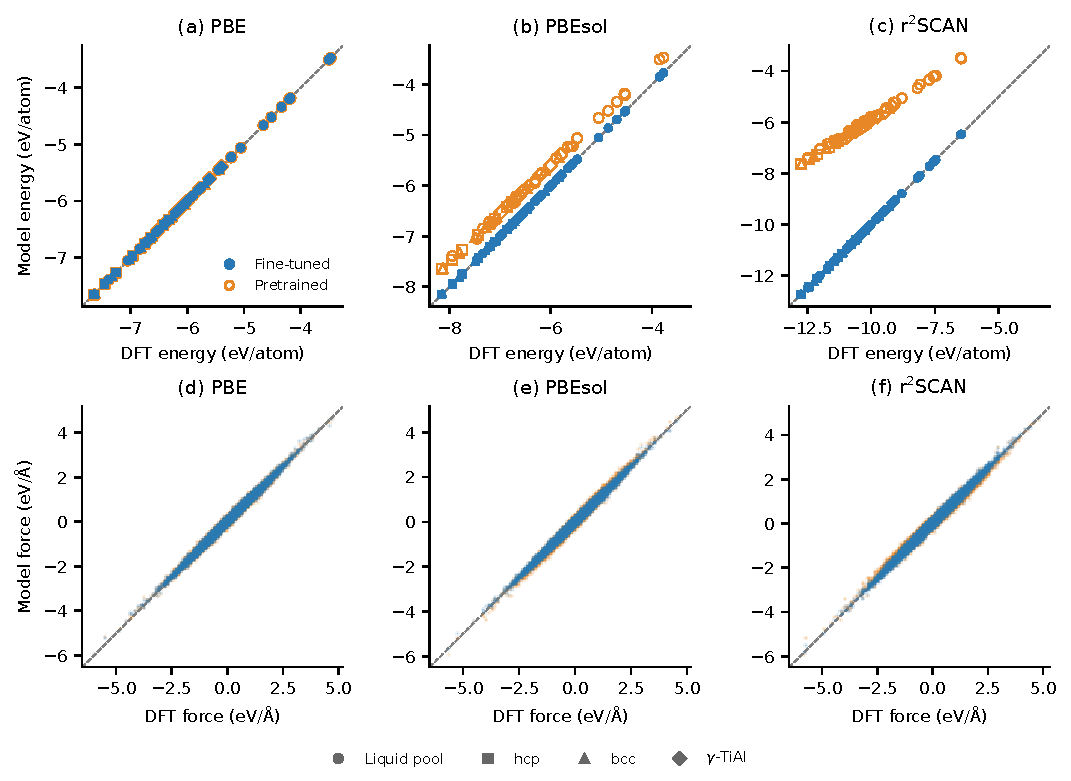
\includegraphics[width=\textwidth]{figures/testset_parity.pdf}
\caption{Parity plots for 49 common geometries from the 50-configuration test design. Panels (a)--(c) compare raw energies per atom and (d)--(f) Cartesian force components against PBE, PBEsol, and \rscan{}, respectively. Blue denotes the fine-tuned model; orange denotes the unchanged pretrained model, with open energy symbols. Marker shapes identify liquid (circles), hcp (squares), bcc (triangles), and $\gamma$-TiAl (diamonds) source families. Force statistics contain 34\,446 components. No energy-reference offsets are fitted or applied.}
\label{fig:test_parity}
\end{figure*}

The fine-tuned energy MAEs are 1.11, 1.48, 1.35~meV/atom for PBE, PBEsol, and \rscan{}, respectively; the corresponding RMSEs are 1.47, 1.77, 1.58~meV/atom.
Descriptive 95\% structure-bootstrap intervals for these RMSEs are 1.1176--1.8233, 1.4684--2.0435, 1.3654--1.7743~meV/atom.
PBE has a mean energy residual of $+0.66$~meV/atom and a largest absolute residual of 4.42~meV/atom.
Its energy MAE and RMSE are both smaller than the pretrained values of 2.49 and 2.93~meV/atom.

Fine-tuned force-component RMSEs are 0.0626, 0.0622, 0.0714~eV/\AA, compared with 0.0735, 0.0832, 0.1038~eV/\AA{} for the pretrained model against PBE, PBEsol, and \rscan{}, respectively.
The central values decrease by approximately 15\%, 25\%, 31\% after fine-tuning.
The force-RMSE bootstrap intervals are 0.0582--0.0669, 0.0578--0.0665, 0.0661--0.0765~eV/\AA; their overlap cautions against a strong ranking of the three fits.
Stress RMSEs are 0.072, 0.070, 0.073~GPa.
These pooled Cartesian-component errors differ from the force-vector quantities printed in the training logs.

Raw pretrained energy RMSEs are approximately 427~meV/atom against PBEsol and 4254~meV/atom against \rscan{}.
They include differences in elemental energy references and exchange-correlation descriptions, and therefore do not measure configuration-dependent errors alone.
Force and stress comparisons provide complementary evidence because constant elemental energy shifts leave these derivatives unchanged.

\subsection{Lattice dynamics and thermal density of Ti}
\label{sec:results_crystal}

Figure~\ref{fig:phonons} compares the harmonic response of $\alpha$-Ti at two levels.
The left column shows direct DFT and corresponding fine-tuned DPA4 dispersions against experiment; the right column compares their DOS.
Because the two calculations within each functional use the same DFT-relaxed geometry and phonon protocol, DFT--experiment discrepancies can be assessed separately from the additional DPA4--DFT mismatch.
All six spectra have no frequencies below $-10^{-3}$~THz on the sampled path or phonon mesh, consistent with harmonic stability within this sampling.

The direct DFT curves show that the functional ranking depends on the branch and wave vector.
Near $\Gamma$, the experimental optical features lie at approximately 4.1 and 5.5~THz.
PBE gives an optical doublet at 3.964~THz and a nondegenerate mode at 5.408~THz, closer to these features than the corresponding PBEsol values of 3.786 and 5.758~THz or the \rscan{} values of 4.587 and 5.189~THz.
The higher \rscan{} optical branches around K also lie above the experimental points near 7~THz.
These discrepancies are already present in the direct electronic-structure calculations and therefore cannot be attributed to fine-tuning.
The direct comparison does not support a uniform improvement of the experimental dispersion on replacing a GGA with \rscan{}.
This is a comparison of static harmonic predictions with room-temperature measurements; it is not a separation of exchange-correlation error from thermal and numerical effects.

\begin{figure*}[t]
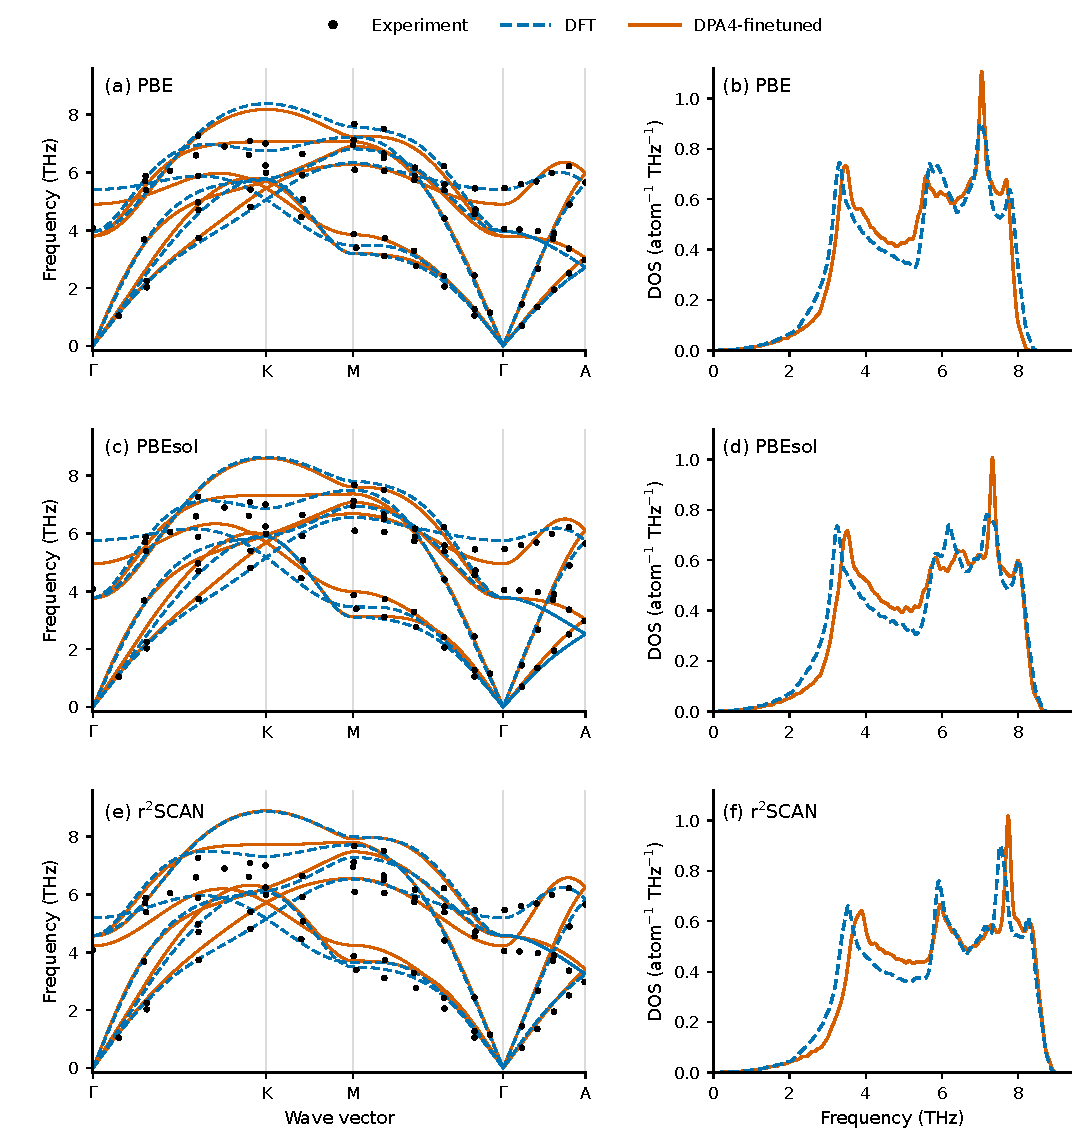
\includegraphics[width=\textwidth]{figures/phonons_alpha_ti.pdf}
\caption{Harmonic dispersions (left) and densities of states (right) of $\alpha$-Ti: PBE (a,b), PBEsol (c,d), and \rscan{} (e,f). Black points are the same 77 digitized room-temperature measurements reproduced in Ref.~\onlinecite{Souvatzis2007}, attributed there to Stassis \textit{et al.} Blue dashed curves denote direct DFT; orange solid curves denote the corresponding DPA4-finetuned model. Each pair uses the same functional-specific DFT-relaxed cell, $4\times4\times3$ supercell, $\pm0.01$~\AA{} displacements, and Phonopy processing. DOS curves use a $\Gamma$-centered $50^3$ mesh and $\sigma=0.05$~THz broadening, with three modes per atom. The calculations use the numerical settings in Sec.~\ref{sec:phonons}; DFT convergence tests remain pending.}
\label{fig:phonons}
\end{figure*}

The DPA4 curves broadly reproduce the DFT dispersion shapes, but leave systematic optical-mode errors.
The nondegenerate optical frequency at $\Gamma$ decreases from 5.408 to 4.903~THz for PBE, from 5.758 to 4.954~THz for PBEsol, and from 5.189 to 4.221~THz for \rscan{}.
The last change reverses its ordering relative to the optical doublet, which remains close to DFT (4.563 versus 4.587~THz).
Thus, the rearrangement of the \rscan{} optical modes in the fine-tuned model is mainly a representation error of that nondegenerate mode, rather than an intrinsic prediction of the reference functional.
The root-mean-square DPA4--DFT differences of frequency-ordered eigenvalues along the plotted path are 0.209, 0.278, and 0.259~THz for PBE, PBEsol, and \rscan{}, respectively.
These are descriptive spectral discrepancies at the sampled wave vectors, without polarization tracking through crossings; they are not errors relative to experiment.

The DOS panels expose additional differences in the distribution of modes even where the dispersion curves appear close.
For example, the principal PBEsol peak between 7 and 8~THz shifts from 7.194~THz in DFT to 7.328~THz in DPA4, while its height increases from 0.782 to 1.007~modes/(atom\,THz).
The corresponding \rscan{} peak shifts from 7.538 to 7.744~THz.
These changes persist with identical geometry, sampling, broadening, and normalization, and therefore reflect differences in the calculated force constants rather than plotting conventions.
Agreement with experiment alone would not expose all such errors: a model shift can either increase or partially cancel the DFT--experiment discrepancy.

The retained $\alpha_2$-Ti$_3$Al model calculations likewise have no appreciable imaginary frequencies along the sampled $\Gamma$--M--K--$\Gamma$--A--L--H--A path; the largest residual negative magnitude is below $10^{-3}$~THz.
Their maximum frequencies are 9.14, 9.48, and 9.58~THz for PBE, PBEsol, and \rscan{}, respectively.
These results characterize model differences for the compound; the matched DFT/DPA4 and experimental comparisons in Fig.~\ref{fig:phonons} concern elemental $\alpha$-Ti.
Neither the harmonic calculations nor the room-temperature comparison determine the temperature-renormalized phonon spectrum near melting.

The temperature-dependent density of elemental Ti provides a complementary test of the equilibrium volume (Fig.~\ref{fig:density_ti}).
At 300~K, PBE 15k and \rscan{} give similar densities, 4.553 and 4.565~g/cm$^3$, whereas PBEsol gives 4.737~g/cm$^3$; the retained PBE 5k value is 4.559~g/cm$^3$.
The solid-state reference is the tabulation by Zinov'ev,\cite{Zinoviev1989} obtained from thermal-expansion data and the room-temperature density.
Relative to its 300~K value of 4.50~g/cm$^3$, the deviations are approximately $+1.2\%$, $+1.5\%$, and $+5.3\%$ for PBE 15k, \rscan{}, and PBEsol, respectively.
The higher PBEsol density persists over the temperature range considered.
The crystalline branches were obtained from separately prepared $\alpha$-Ti and $\beta$-Ti cells at 300--1100 and 1200--1900~K, respectively, rather than by heating a single crystal through the $\alpha$--$\beta$ transition.
Figure~\ref{fig:density_ti}(a) marks the experimental transition temperatures, approximately 1155~K for $\alpha$--$\beta$ and 1943~K for melting, as reference guides rather than predictions of the models.
The two crystalline phases have very similar densities: the solid-state tabulation gives 4.37 and 4.38~g/cm$^3$ for $\alpha$- and $\beta$-Ti near the transition, a difference of only about 0.2\%.
This small density change is barely visible on the scale of the figure, and the simulated branches likewise show no pronounced discontinuity between the neighboring 1100 and 1200~K points.
The temperature grid does not resolve the transition jump itself.
Within each preparation series the density generally decreases with temperature.
The archived solid-initialized PBE 5k and PBEsol series exhibit a marked decrease between 1600 and 1800~K, while the \rscan{} series retains a higher density at 1800--1900~K.
In the PBE 15k series, the cell initialized as $\beta$-Ti retains crystalline order at 1800~K, with density $4.3632\pm0.0011$~g/cm$^3$, but melts during equilibration at 1900~K, giving $4.2753\pm0.0011$~g/cm$^3$ during liquid production.
Over the last 10~ps, the fraction with $\bar q_6>0.25$ is 0.968 at 1800~K and 0.0004 at 1900~K; the corresponding 10~ps mean-square displacements are 0.77 and 30.30~\AA$^2$.
Persistence of the homogeneous crystal at 1800~K is compatible with metastability above the coexistence melting bracket and does not establish a new equilibrium melting temperature.
This high-temperature decrease is separate from the $\alpha$--$\beta$ transition and motivates the coexistence analysis below, but a density change in a short, initially homogeneous simulation is not itself an equilibrium melting-temperature measurement.

For liquid Ti, we use the experimental reference correlation of Ntonti \textit{et al.},\cite{Ntonti2024}
\begin{equation}
\rho_{\mathrm{ref}}(T)=4.2221-3.952\times10^{-4}(T-1941),
\label{eq:ti_liquid_density_reference}
\end{equation}
where $\rho_{\mathrm{ref}}$ is in g/cm$^3$ and $T$ is in kelvin.
This correlation applies at 0.1~MPa over 1941--3520~K and has a reported expanded uncertainty of 2.0\% at 95\% coverage.
It covers the six liquid temperatures from 2000 to 2500~K without extrapolation; the points at 1873~K lie below its stated range and are not compared with an extrapolated correlation.
Figure~\ref{fig:density_ti}(b) also shows individual liquid-Ti measurements from electromagnetic levitation by Reiplinger and Brillo,\cite{Reiplinger2022} digitized with their reported error bars from the published vector graphic.
These measurements span approximately 1858--2088~K and include undercooled liquid; their experimental error bars are distinct from the expanded uncertainty band of the Ntonti correlation.
The PBE 15k liquid densities are $4.2828\pm0.0008$~g/cm$^3$ at 1873~K and $4.2606\pm0.0011$~g/cm$^3$ at 2000~K, with block standard errors.
The completed PBE 15k recalculations give $4.2415\pm0.0012$, $4.2247\pm0.0011$, $4.2064\pm0.0009$, $4.1899\pm0.0008$, and $4.1717\pm0.0015$~g/cm$^3$ at 2100, 2200, 2300, 2400, and 2500~K, respectively, forming a monotonically decreasing series.
Their mean logged pressures range from 8.11 to 9.71~MPa despite the 0.1~MPa target; the block SEM describes sampling uncertainty and does not include this residual protocol bias.
The PBEsol and \rscan{} liquid branches now use 90~ps production at each temperature, replacing the earlier 30~ps estimates and adding 1873~K.
At 1873~K, the densities are $4.4830\pm0.0006$~g/cm$^3$ for PBEsol and $4.3368\pm0.0007$~g/cm$^3$ for \rscan{}; at 2500~K they are $4.3765\pm0.0008$ and $4.2355\pm0.0007$~g/cm$^3$, respectively.
Both extended series decrease monotonically without fitted smoothing. Diffusion and local-order diagnostics support liquid behavior throughout production, including at 1873~K; this does not determine an equilibrium melting boundary.
Their mean pressures are 7.22--10.47~MPa, with block 95\% intervals excluding the 0.1~MPa target at every point. The density SEM does not include this protocol limitation.
At 2000~K, the reference correlation gives 4.199~g/cm$^3$, compared with 4.261, 4.316, and 4.461~g/cm$^3$ for PBE 15k, \rscan{}, and PBEsol: deviations of $+1.5\%$, $+2.8\%$, and $+6.2\%$.
The 2100--2500~K series decrease less steeply with temperature than the reference; at 2500~K the deviations are $+4.3\%$ for PBE 15k, $+4.4\%$ for PBE 5k, $+5.9\%$ for \rscan{}, and $+9.4\%$ for PBEsol.
PBE remains closest to the central reference in this high-temperature comparison; the PBE 15k value at 2000~K lies within the reference uncertainty band.
The original PBE 5k points remain visible alongside completed 15k calculations. Their difference includes sensitivity to the recording interval and should not be attributed solely to the checkpoint change.
Thus, the liquid-density comparison does not support a uniform advantage of \rscan{} over PBE.
This ordering describes deviations from the central correlation and does not by itself establish statistical separation of the models.

\begin{figure*}[t]
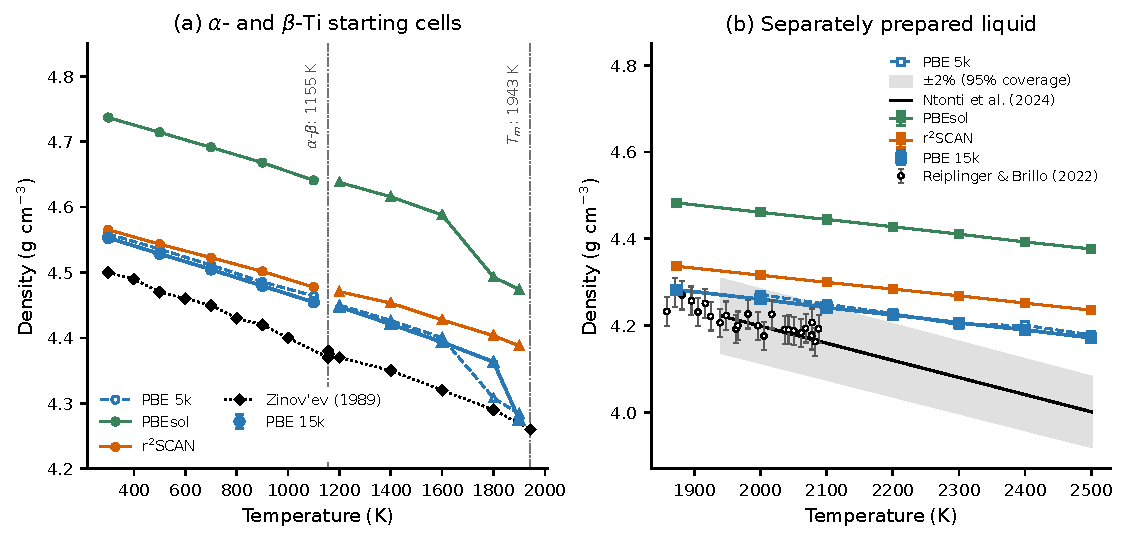
\includegraphics[width=\textwidth]{figures/density_ti_6e45e69b79dc.pdf}
\caption{Temperature-dependent density of elemental Ti compared with experiment. (a) Circles and triangles denote simulations initialized from separately prepared $\alpha$-Ti and $\beta$-Ti cells, respectively; these symbols specify preparation, not persistence of the crystalline phase. The PBE 15k cell initialized as $\beta$-Ti at 1900~K is liquid during production. Vertical lines mark the experimental $\alpha$--$\beta$ transition (approximately 1155~K) and melting (1943~K). Black diamonds are the solid densities in Table~65 of Zinov'ev,\cite{Zinoviev1989} derived from thermal expansion and room-temperature density; dotted lines connect values within each phase. (b) Separately prepared liquids (colored squares). Open black circles and error bars are measurements from Fig.~4 of Reiplinger and Brillo,\cite{Reiplinger2022} digitized from the published graphic, including undercooled liquid. The black line is the Ntonti \textit{et al.}\cite{Ntonti2024} correlation, shown within its stated temperature range; shading is its $\pm2\%$ expanded uncertainty at 95\% coverage. This band is distinct from the measurement error bars and does not describe MLIP uncertainty. Open blue symbols and dashed lines retain all PBE 5k points; filled blue symbols show completed PBE 15k points with block SEM bars. Blue solid segments join adjacent completed temperatures within the same preparation series. PBEsol and \rscan{} in (b) use 90~ps production at 1873~K and 2000--2500~K, sampled every 10~fs, with block SEM bars; their solid-initialized series in (a) are unchanged. Colored solid lines connect sampled means without fitted smoothing. SEM bars exclude protocol and model uncertainties.}
\label{fig:density_ti}
\end{figure*}

\subsection{Solid--liquid coexistence and melting}
\label{sec:results_melting}

The coexistence trajectories provide a clearer distinction between the models.
Figure~\ref{fig:melting} shows the evolution of the solid-like atom fraction near the temperature at which the direction of interface motion changes.
For PBE, the crystal grows at 1750~K and the liquid layer ceases to be resolved at approximately 11~ps.
At 1775~K, both interfaces retreat into the solid, which disappears at approximately 12~ps; the system remains liquid through 100~ps.
The 1800~K trajectory also melts, with the crystalline layer disappearing at approximately 13.5~ps.
Opposite single-phase outcomes therefore give a working bracket of 1750--1775~K.

For PBEsol, crystallization occurs at 1730~K and complete melting at 1770~K.
At 1750~K, the solid fraction fluctuates and decreases overall, but the solid slab survives to the end of the run.
We therefore retain 1730--1770~K as the conservative bracket.
The \rscan{} trajectories yield a narrower observed bracket: the crystal grows in both preparations at 1850~K, whereas the solid layer disappears at 1860~K.
Changing the structural-order threshold or using the bond-correlation criterion preserves the principal distinction between growth and retreat.

\begin{figure*}[t]
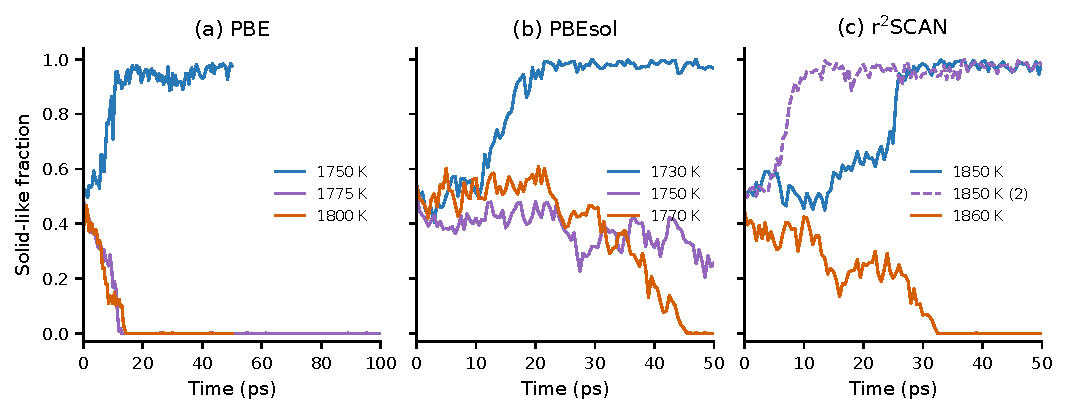
\includegraphics[width=\textwidth]{figures/melting_ti.pdf}
\caption{Solid-like fraction in representative 1296-atom Ti coexistence trajectories, using $\bar q_6>0.25$. For PBE, the 1775~K trajectory extends to 100~ps and the 1750/1800~K trajectories to 50~ps. PBEsol and \rscan{} trajectories are 50~ps long; panel time ranges differ accordingly. The two \rscan{} trajectories at 1850~K have different preparation histories; the dashed curve denotes the second preparation. The fraction diagnoses growth or retreat of the crystalline slab, rather than an exact thermodynamic phase fraction.}
\label{fig:melting}
\end{figure*}

\begin{table}[tb]
\caption{Ti melting estimates and brackets from opposite single-phase outcomes. PBE uses 50~ps at 1750~K and 100~ps at 1775~K; the other models use 50~ps trajectories. The PBE estimate is a rounded representative value within its 25~K bracket. The reference value is 1943~K, as used in Ref.~\onlinecite{Wang2012}. Brackets are protocol-dependent observations, not confidence intervals.}
\label{tab:melting}
\begin{ruledtabular}
\begin{tabular}{lrrr}
Model & Estimate (K) & Bracket (K) & Bias (\%)\\
\hline
PBE  & $\sim1760$ & 1750--1775 & $-9.4$\\
PBEsol   & $\sim1750$ & 1730--1770 & $-9.9$\\
\rscan{} & $\sim1855$ & 1850--1860 & $-4.5$\\
\end{tabular}
\end{ruledtabular}
\end{table}

The working estimates are approximately 1760, 1750, and 1855~K for PBE, PBEsol, and \rscan{}, respectively (Table~\ref{tab:melting}).
Relative to 1943~K, the \rscan{} model reduces the underestimation from about 180--190~K to 88~K.
Using 1941~K as the experimental reference would not change this ranking.
The approximately 100~K separation between \rscan{} and the two GGA-based potentials exceeds the widths of their observed brackets.
This makes melting the clearest improvement obtained with \rscan{} in the present set of tests.
The 1850--1860~K bracket must nevertheless not be interpreted as a total uncertainty of $\pm5$~K: finite cell size, interface interactions, preparation dependence, and finite observation time remain unquantified.

\subsection{Liquid density and mixing thermodynamics}
\label{sec:results_thermo}

We next compare properties across composition, using $x_{\mathrm{Al}}=N_{\mathrm{Al}}/(N_{\mathrm{Al}}+N_{\mathrm{Ti}})$ throughout.
At 1873~K, all models predict a monotonic decrease in density as Ti is replaced by Al (Fig.~\ref{fig:liquid_density}).
PBE gives the lowest densities and PBEsol generally the highest, with \rscan{} between them.
The comparison uses the densities tabulated at 1873~K by Brillo \textit{et al.}\cite{Brillo2025}
PBE is closest overall to this reference set.
Using equal weight for each of the 11 common compositions and averaging multiple published entries at the same composition gives mean absolute deviations of 0.112, 0.246, and 0.189~g/cm$^3$ for PBE, PBEsol, and \rscan{}, respectively.
The corresponding mean absolute relative deviations are 3.3\%, 7.5\%, and 5.8\%.
These are descriptive discrepancies against the tabulated values, rather than statistically weighted goodness-of-fit measures.

\begin{figure*}[t]
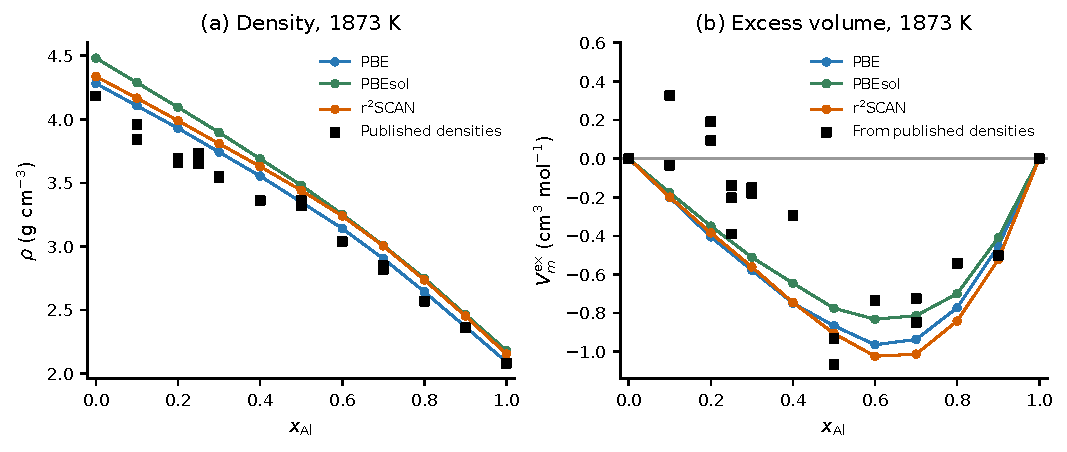
\includegraphics[width=\textwidth]{figures/liquid_density.pdf}
\caption{Liquid density (a) and excess molar volume (b) at 1873~K. The PBE series uses 30~ps production after 30~ps equilibration; PBEsol and \rscan{} retain their original series. Black symbols in (a) are the printed densities in Table~7 of Ref.~\onlinecite{Brillo2025}; separate entries at the same composition are shown individually. Reference excess volumes in (b) are recomputed from those densities and their pure-component endpoints. Each MLIP excess volume uses its own pure-liquid references. Some experimental reference values represent extrapolated or undercooled-liquid states.}
\label{fig:liquid_density}
\end{figure*}

All three models predict negative excess molar volumes at the sampled interior compositions.
At 1873~K, the discrete minima are approximately $-0.96$~cm$^3$/mol at $x_{\mathrm{Al}}=0.6$ for PBE, $-0.83$~cm$^3$/mol at $x_{\mathrm{Al}}=0.6$ for PBEsol, and $-1.02$~cm$^3$/mol at $x_{\mathrm{Al}}=0.6$ for \rscan{}.
Thus, mixing produces substantial volume contraction relative to each model's pure-liquid reference volumes.
The published densities also imply a pronounced contraction over much of the intermediate and Al-rich composition range, but yield appreciable scatter and positive excess volumes at some Ti-rich compositions.
The models therefore capture the principal contraction without reproducing all features of the reference data.
Absolute density and excess volume probe different combinations of pure-component and alloy errors; agreement in one does not guarantee agreement in the other.

\draftnote{The density comparison currently uses the printed 1873~K column of Table~7 in Ref.~\onlinecite{Brillo2025}. At least one equiatomic entry is inconsistent with its listed temperature-fit coefficients. Resolve the reference convention before finalizing numerical error metrics. Some values are extrapolated, and Ti-rich liquids at 1873~K are below the experimental liquidus.}

The mixing enthalpy gives a different ranking (Fig.~\ref{fig:mixing}).
At 2000~K, all three models predict strongly exothermic mixing and a broad minimum near intermediate composition.
The PBE and PBEsol minima are $-25.0$ and $-25.4$~kJ/mol at $x_{\mathrm{Al}}=0.5$.
The extended 60~ps \rscan{} series gives $-31.66\pm0.19$~kJ/mol at $x_{\mathrm{Al}}=0.5$ and $-31.74\pm0.20$~kJ/mol at 0.6.
Although the latter is the numerical minimum, their difference is only $-0.081\pm0.263$~kJ/mol, including the shared pure-component covariance, so its position is not resolved between these compositions.
The PBE minimum is $-25.01\pm0.30$~kJ/mol.
The quoted errors are propagated block standard errors; the longer \rscan{} sampling changes the mean curve by at most 0.39~kJ/mol and does not uniformly reduce these errors.
The values reported here use the thermodynamic enthalpy at the imposed external pressure, as defined in Sec.~\ref{sec:thermodynamics}, and consistent pure-liquid reference calculations.

The experimental comparison is based on calorimetric points reproduced in Fig.~7 of Witusiewicz \textit{et al.}\cite{Witusiewicz2008}
Their CALPHAD curve is not used as an experimental dataset.
The reproduced points indicate a minimum of approximately $-29.5$ to $-30$~kJ/mol near $x_{\mathrm{Al}}=0.5$--0.6.
PBE and PBEsol underestimate the depth of this minimum, whereas \rscan{} overestimates it.
Across nine digitized interior compositions, the provisional mean absolute deviations are approximately 3.6, 3.1, and 1.5~kJ/mol for PBE, PBEsol, and \rscan{}, respectively.
Consequently, \rscan{} better reproduces the overall composition dependence under this metric, although it is not uniformly closer at every composition.

\begin{figure}[htbp]
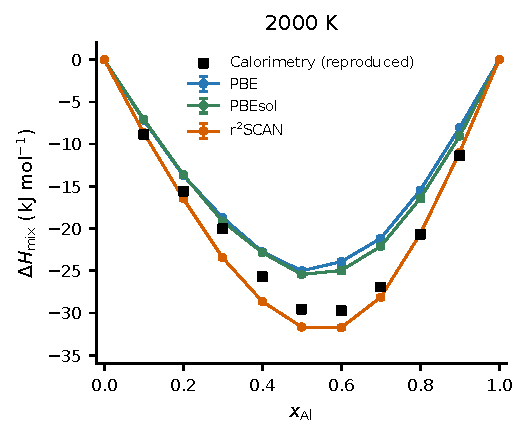
\includegraphics[width=\columnwidth]{figures/mixing_enthalpy.pdf}
\caption{Liquid mixing enthalpy at 2000~K compared with calorimetric points reproduced in Ref.~\onlinecite{Witusiewicz2008}. Reference points are a provisional digitization of calorimetric symbols. PBE error bars propagate the maximum block SEM over 3, 5, and 6~ps blocks; PBEsol uses six 5~ps blocks and \rscan{} uses twelve 5~ps blocks from 60~ps production. Both pure-liquid references are included. These are diagnostic standard errors, not final confidence intervals. Lines connect sampled compositions.}
\label{fig:mixing}
\end{figure}

These results quantify a difference in the energetic preference for the alloy relative to its pure liquids.
They do not, by themselves, identify a particular electronic mechanism or establish chemical short-range order.

\draftnote{The original calorimetric reports behind Ref.~\onlinecite{Witusiewicz2008} are unavailable. The current digitization has an estimated reading tolerance of about 0.2~kJ/mol, which is not an experimental uncertainty. Finalize the digitization and trajectory uncertainty analysis before treating the quoted deviations as publication-ready metrics.}

\subsection{Liquid viscosity}
\label{sec:results_viscosity}

Both potentials predict a nonmonotonic composition dependence of liquid viscosity at 1873~K (Fig.~\ref{fig:viscosity}a).
Adding Al initially increases the viscosity, producing a broad maximum at intermediate composition, followed by a pronounced decrease toward the Al-rich end.
The largest sampled values are $5.02\pm0.19$~mPa\,s at $x_{\mathrm{Al}}=0.40$ for PBE and $7.19\pm0.28$~mPa\,s at $x_{\mathrm{Al}}=0.45$ for \rscan{}.
The neighboring compositions have similar viscosities, so neither curve locates a sharp maximum.
The \rscan{} values exceed those of PBE at all eleven sampled compositions.

\begin{figure*}[t]
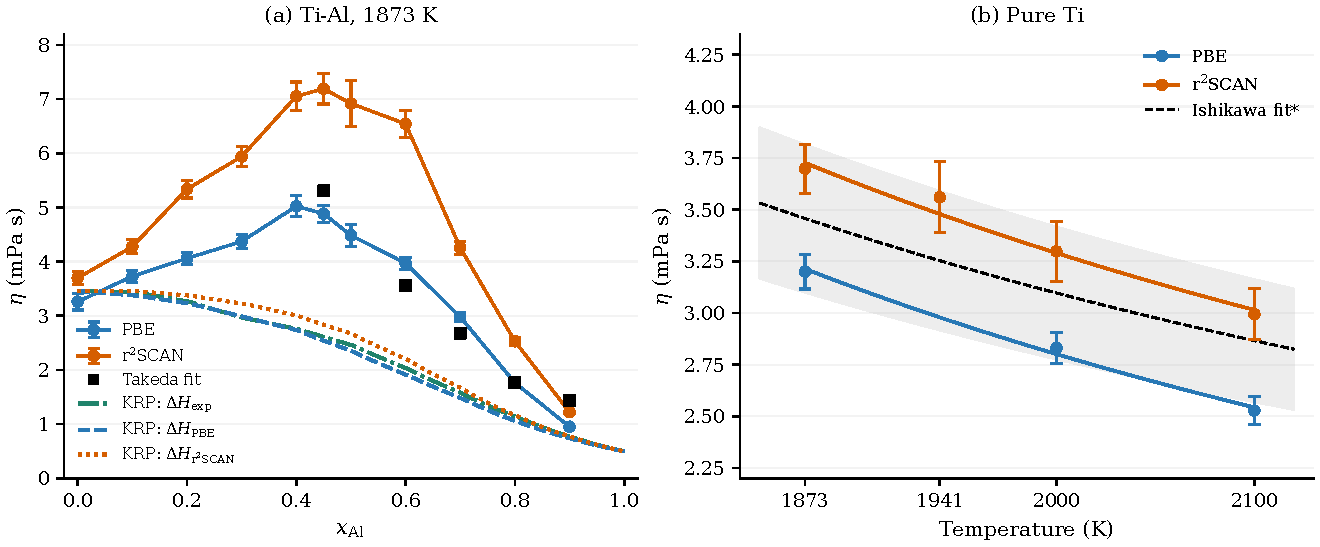
\includegraphics[width=\textwidth]{figures/viscosity.pdf}
\caption{Liquid viscosity versus Al mole fraction at 1873~K (a) and temperature for pure Ti (b). Colored symbols show the PBE and \rscan{} estimates with estimator standard errors. Solid lines in (a) connect sampled compositions; solid colored curves in (b) are weighted Arrhenius fits. Black squares in (a) are values from the experimental correlations of Takeda \textit{et al.}\cite{Takeda2025} Additional lines in (a) show the KRP model with calorimetric (green dash-dotted), PBE (blue dashed), and \rscan{} (orange dotted) mixing enthalpies. All three use the Ishikawa pure-Ti viscosity and the extrapolated Assael pure-Al correlation.\cite{Assael2006} MD enthalpies are at 1873~K; calorimetry at 2000~K is transferred without a temperature correction (Sec.~\ref{sec:viscosity}). The dashed curve marked with an asterisk in (b) is a provisional transcription of the Ishikawa \textit{et al.}\cite{Ishikawa2012} correlation; the shaded band denotes its reported 10.3\% uncertainty.}
\label{fig:viscosity}
\end{figure*}

PBE is closer to the experimental alloy-viscosity correlations at four of the five compared compositions: $x_{\mathrm{Al}}=0.45$, 0.60, 0.70, and 0.80.
At $x_{\mathrm{Al}}=0.45$, the experimental reference is 5.30~mPa\,s, compared with 4.88 for PBE and 7.19 for \rscan{}.
At $x_{\mathrm{Al}}=0.80$, the corresponding values are 1.764, 1.761, and 2.528~mPa\,s.
The Al-rich state at $x_{\mathrm{Al}}=0.90$ is an exception: \rscan{} gives 1.218~mPa\,s, closer to the reference value of 1.437~mPa\,s than the PBE result of 0.951~mPa\,s.
The two lowest-composition reference values involve a small, 3~K extrapolation of the experimental correlations to 1873~K.
No alloy-viscosity reference is available below $x_{\mathrm{Al}}=0.45$, so the predicted increase on the Ti-rich side cannot be tested by this dataset.

With the common experimental pure-component inputs specified in Sec.~\ref{sec:viscosity}, the three KRP curves do not reproduce the pronounced intermediate-composition viscosity maximum.
At $x_{\rm Al}=0.45$, Eq.~\eqref{eq:krp} gives 2.61, 2.54, and 2.83~mPa\,s using the calorimetric, PBE, and \rscan{} mixing enthalpies, respectively, compared with the experimental correlation value of 5.30~mPa\,s.
Thus, changing the enthalpy input alone within these datasets does not recover the observed enhancement; this comparison remains conditional on the extrapolated pure-Al viscosity and, for the calorimetric curve, the neglect of the enthalpy temperature dependence.

For pure Ti, both potentials predict decreasing viscosity with increasing temperature (Fig.~\ref{fig:viscosity}b).
The PBE estimates decrease from $3.200\pm0.084$~mPa\,s at 1873~K to $2.528\pm0.068$~mPa\,s at 2100~K, while the \rscan{} values decrease from $3.70\pm0.12$ to $2.99\pm0.12$~mPa\,s.
Both series are consistent with smooth Arrhenius temperature dependences within the reported errors.
In particular, the deviations of individual \rscan{} points from the fitted curve do not resolve a change in slope or an anomalous temperature dependence.
Relative to the experimental correlation, PBE and \rscan{} lie on opposite sides at 1873~K, with deviations of approximately $-7.4\%$ and $+7.0\%$, respectively.
At 2000 and 2100~K, \rscan{} is closer to the central experimental correlation.
Thus, the advantage of PBE for most of the compared alloy compositions does not extend uniformly to pure-Ti viscosity over the studied temperature range.

Taken together, the present benchmarks show that the benefit of changing the reference functional depends on the observable.
The \rscan{} potential raises the Ti melting temperature toward experiment and improves the overall mixing-enthalpy comparison, but these gains do not extend uniformly to lattice dynamics, liquid density, or viscosity.
The different rankings are the central outcome of the multi-property assessment and motivate a separate discussion of reference-functional effects, residual fitting errors, and sampling limitations.

\section{Discussion}
\label{sec:discussion}

The most consistent gains obtained with \rscan{} concern two thermodynamic differences: the balance between solid and liquid Ti, and the enthalpy of an alloy liquid relative to its pure components.
The melting estimate moves toward experiment, and the overall mixing-enthalpy discrepancy decreases, although the broad minimum near equiatomic composition becomes too deep.
Density, phonons, and viscosity do not follow the same ranking.
These observations suggest that the benefit of \rscan{} is associated with how it distinguishes competing atomic environments, rather than with a uniform improvement of all features of the potential-energy surface.

\subsection{The solid--liquid free-energy balance}

At fixed pressure, melting occurs when the Gibbs free energies of the solid and liquid are equal.
Let $g_s^A$ and $g_l^A$ denote these free energies per atom for a reference potential $A$, and let $\delta g_i=g_i^B-g_i^A$ be the change on replacing it by potential $B$.
Linearization about the melting point of $A$ gives
\begin{equation}
 \delta T_m \simeq
 \frac{\delta g_l(T_m^A,p)-\delta g_s(T_m^A,p)}
 {\Delta s_{\mathrm{fus}}^A},
 \label{eq:melting_shift}
\end{equation}
where $\Delta s_{\mathrm{fus}}^A=s_l^A-s_s^A>0$ is the entropy of fusion per atom, evaluated at that point.
Thus, a positive change in the liquid--solid free-energy difference raises the melting temperature.
The approximately 95~K increase from the representative PBE estimate to \rscan{} is consistent with greater relative stability of the crystal near coexistence.
It does not determine whether this change is predominantly energetic or entropic, since both contributions enter $g_l-g_s$.
We have not calculated the fusion enthalpy or entropy separately and therefore do not assign a numerical free-energy correction to this temperature shift.

This distinction is particularly relevant for Ti.
Its high-temperature bcc phase is stabilized by finite-temperature lattice dynamics, which cannot be described by the unstable zero-temperature harmonic spectrum alone.\cite{Souvatzis2008}
Our coexistence calculations start from a bcc slab and sample ionic motion explicitly.
Their melting behavior depends on the full potential-energy surface explored by the two phases, including anharmonic contributions.
The harmonic $\alpha$-Ti spectra characterize a different phase and a local curvature of that surface.
Their mixed ranking is therefore compatible with the clearer improvement of the \rscan{} melting estimate.

The density results likewise show why a simple association between a smaller equilibrium volume and a higher melting point is insufficient.
PBEsol gives the largest Ti densities but the lowest working melting estimate, whereas the PBE and \rscan{} densities at 300~K are nearly identical. The PBE and \rscan{} models also differ appreciably in melting temperature despite much smaller relative differences in liquid density.
Volume probes the pressure derivative of the free energy; melting probes the difference between two free energies.
Errors in these quantities need not vary together.
Related sensitivity of melting predictions to the reference functional has been demonstrated in first-principles calculations accelerated by machine-learned force fields.\cite{Jinnouchi2019}
Here, the remaining underestimation of approximately 88~K by \rscan{} also shows that its improved balance is still imperfect.

\subsection{Mixing energetics and a possible electronic origin}

The mixing enthalpy isolates another difference between environments.
Defining $\delta H_m=H_m^B-H_m^A$ at common temperature and pressure, Eq.~\eqref{eq:mixing} gives
\begin{align}
 \delta\Delta H_{\mathrm{mix}}(x)={}&\delta H_m(x)
 -x\,\delta H_m^{\mathrm{Al}}\nonumber\\
 &-(1-x)\,\delta H_m^{\mathrm{Ti}}.
 \label{eq:mixing_shift}
\end{align}
Any constant energy offsets assigned separately to Ti and Al cancel in this expression.
The change therefore reflects the treatment of alloy environments relative to the elemental liquids, including the different structures sampled by the models.
At $x=0.5$ and 2000~K, replacing PBE by \rscan{} lowers the calculated mixing enthalpy by approximately 6.65~kJ/mol, or 69~meV/atom.
This is a substantial change in the energetic preference for mixing.
It brings much of the composition curve closer to the reproduced calorimetric points, while overshooting their minimum.
The provisional overall improvement consequently supports a more favorable description of this particular energy difference, without implying that increasingly exothermic mixing is always more accurate.

The construction of \rscan{} offers a plausible reason for changes of this kind.
Unlike a GGA, the SCAN family uses the orbital kinetic-energy density in addition to the electron density and its gradient.
This extra ingredient distinguishes electronic environments associated with different bonding regimes.\cite{Sun2015}
The regularization and constraint restoration in \rscan{} improve numerical behavior while retaining much of this flexibility.\cite{Furness2020}
In Ti--Al, changes in chemical coordination and crystal order can therefore receive different exchange-correlation corrections even when average density changes are modest.
This provides a physical basis for expecting shifts in relative energies, but does not prescribe their sign or guarantee improved agreement.

Existing electronic-structure studies illustrate why Ti environments deserve particular attention.
Calculations for crystalline TiAl find a substantial Ti-$3d$ contribution near the Fermi level.\cite{Hussain2011}
Moreover, Song \textit{et al.}\cite{Song1994} found that the alternating Ti and Al planes in $\gamma$-TiAl strengthen particular directional Ti--Ti bonding states relative to hypothetical fcc Ti.
Thus, adding Al can modify the Ti-derived bonding network as well as introduce unlike neighbors.
Changes in Ti--Al hybridization and Ti--Ti bonding are plausible microscopic contributions to the functional dependence of mixing.
The crystalline results motivate this interpretation; they do not establish that the same redistribution persists in a disordered liquid.
Our thermodynamic data contain no direct measurement of orbital occupations, charge transfer, or bond-resolved energies.
An attribution of the \rscan{} improvement to a specific electronic redistribution therefore remains a hypothesis.

The two favorable thermodynamic shifts also cannot be reduced to a single assertion of stronger bonding.
Raising the melting point of pure Ti concerns environments containing only Ti, whereas making alloy mixing more exothermic concerns the alloy relative to both elemental liquids.
Neither shift logically requires the other.
Their coexistence is consistent with improved environment-dependent energy differences, but a common microscopic cause has not been demonstrated.
Broad benchmarks reinforce this qualification: \rscan{} improves many solid-state formation enthalpies, yet PBE remains competitive and can have smaller average errors for intermetallic subsets.\cite{Kothakonda2023}
Those benchmarks concern crystalline formation energies, rather than liquid mixing, but show that the meta-GGA level alone does not establish superiority for a given alloy.

\subsection{Separating reference and representation errors}

The paired phonon calculations make this distinction explicit for the local curvature of the $\alpha$-Ti potential-energy surface.
Direct DFT--experiment comparisons assess the three electronic-structure descriptions without an intervening learned potential.
The corresponding DPA4--DFT comparisons, at identical geometry and phonon settings within each functional, test the fidelity of the final fine-tuned models to those references.
Near $\Gamma$, the closer agreement of PBE DFT with the experimental optical frequencies is a property of the reference calculation, whereas the downward shifts of the nondegenerate optical mode in all three DPA4 models identify an additional model discrepancy.
In particular, the reversed optical-mode ordering for the \rscan{} model is absent from its DFT reference.

For an identifiable mode at a given wave vector and the same calculated geometry, the model--experiment frequency residual is the sum of the model--DFT and DFT--experiment residuals.
The two contributions can reinforce or cancel one another.
Consequently, closer agreement of a learned potential with an experimental point does not necessarily imply more faithful reproduction of its training functional.
The DOS comparison provides a complementary test of that fidelity over the Brillouin zone, showing residual changes in peak positions and spectral weight at common broadening and normalization.

This separates the two levels of validation without making either error source exact.
The DFT--experiment residual includes the harmonic approximation, the use of a static equilibrium cell, and unresolved numerical convergence, in addition to the electronic-structure approximation.
The model--DFT residual tests the final fine-tuned representation under the phonon protocol, which differs from the training-label protocol in electronic sampling and smearing.
It does not isolate the optimizer's contribution or establish the improvement over the pretrained model without a corresponding pretrained phonon calculation.
The remaining optical errors therefore motivate more targeted validation of force derivatives near the crystal, even when pooled energy and force errors are small.

\subsection{Consequences for validation and transfer learning}

The other observables help delimit the thermodynamic interpretation.
At 2000~K, PBE is closer than \rscan{} to the central experimental liquid-Ti density correlation; PBE also gives smaller overall discrepancies for the alloy densities at 1873~K.
More exothermic mixing and stronger volume contraction are therefore not sufficient criteria for choosing the most accurate model.
Likewise, the higher alloy viscosity predicted by \rscan{} does not improve agreement at four of the five experimentally covered compositions shared with the PBE calculations; the Al-rich state at $x_{\mathrm{Al}}=0.90$ is an exception.
For pure Ti, however, \rscan{} is closer to the central experimental viscosity correlation at 2000 and 2100~K, while both models give temperature dependences consistent with smooth Arrhenius behavior over the sampled interval.
The transport comparison therefore depends on composition and temperature as well as on the reference functional.
Viscosity depends on the amplitude and relaxation time of stress fluctuations, with additional sensitivity to density and liquid structure.
A more accurate mixing enthalpy alone cannot determine these dynamical quantities.
Chemical short-range order could help connect energetics and transport, but would require partial pair correlations or explicit chemical-order parameters; it is not established by the enthalpy minimum.

This outcome differs from our Al--Cu study, where changing from PBE to \rscan{} improved the composition dependence of viscosity as well as several thermodynamic properties.\cite{Khazieva2024}
Together, the two systems support testing alternative reference functionals, while showing that a favorable ranking in one alloy does not transfer automatically to another.
Foundation-model fine-tuning makes such comparisons practical by using a common starting representation for the separate DFT datasets.
The present work demonstrates this use of DPA4-Neo, without a separate benchmark of training cost against models trained from scratch.

Beyond the matched harmonic comparison, a quantitative attribution of thermodynamic changes to exchange-correlation physics must still separate functional effects from potential-fitting and sampling errors.
The common-geometry benchmark in Sec.~\ref{sec:results_fit} gives comparable energy- and force-error scales for the three fits, but these pooled errors do not constrain systematic solid--liquid free-energy biases directly.
This cautions against attributing every property difference to the reference functional alone.
Further targeted tests should include common snapshots of hot bcc Ti and the liquid states relevant to coexistence.
Comparisons at common geometry and volume would isolate electronic-energy and stress changes; separate equilibrium ensembles would reveal the contribution of structural relaxation.
Free-energy perturbation or thermodynamic integration, with adequate ensemble overlap, could then test the melting interpretation in Eq.~\eqref{eq:melting_shift}.
Ensemble-averaged projected densities of states and bond-resolved analyses could examine the proposed electronic origin, but would need to be related to these energy differences.

These checks would refine the causal interpretation.
The coexistence and liquid-density calculations show a property-dependent pattern: \rscan{} improves the Ti coexistence melting estimate and the provisional overall mixing-enthalpy comparison, whereas PBE is closer to the available liquid-density references.
The pure-Ti viscosity comparison does not establish a uniform transport ranking.
The finite-size and observation-time limitations of coexistence, the indirect calorimetric reference, and the sampling uncertainty in viscosity set the precision with which this pattern can presently be quantified.

\section{Conclusions}
\label{sec:conclusions}

We developed Ti--Al interatomic potentials by fine-tuning DPA4-Neo on PBE, PBEsol, and \rscan{} datasets derived from a common pool of selected configurations.
Their comparison across lattice dynamics, density, melting, mixing thermodynamics, and viscosity shows that exchange-correlation choices have property-dependent consequences.
The DFT-reference benchmark gives energy RMSEs of 1.47, 1.77, and 1.58~meV/atom for PBE, PBEsol, and \rscan{}, respectively, with force RMSEs of 0.062--0.071~eV/\AA.
These fitting errors provide context for the property comparison, but do not determine the errors in phase free-energy differences.

The clearest improvement with \rscan{} is the melting temperature of Ti.
PBE trajectories crystallize at 1750~K and melt at 1775~K, giving a working bracket of 1750--1775~K.
Representative melting estimates are approximately 1760~K for PBE, 1750~K for PBEsol, and 1855~K for \rscan{}, reducing the discrepancy from experiment from about 9--10\% to 4.5\%.
These brackets are finite-size and finite-time observations, not confidence intervals.
For liquid mixing at 2000~K, the extended 60~ps \rscan{} series has the smallest provisional overall discrepancy from the reproduced calorimetric data, approximately 1.5~kJ/mol compared with 3.6 and 3.1~kJ/mol for PBE and PBEsol.
Its broad minimum at $x_{\mathrm{Al}}=0.5$--0.6 remains too exothermic; the two sampled compositions are not statistically distinguished as the location of the minimum.

The gains are selective.
PBE is closer overall to the tabulated liquid densities at 1873~K, with a mean absolute deviation of 0.112~g/cm$^3$, compared with 0.246 and 0.189~g/cm$^3$ for PBEsol and \rscan{}.
PBE also gives closer alloy viscosities at four of the five compared compositions; the Al-rich state at $x_{\mathrm{Al}}=0.90$ is the exception.
For pure Ti, both models give temperature dependences consistent with Arrhenius behavior over 1873--2100~K, and \rscan{} is closer to the central experimental viscosity correlation at 2000 and 2100~K.
Neither the viscosity results across these liquid states nor the experimental phonon dispersions therefore provide a uniform ranking of the functionals.

The matched $\alpha$-Ti phonon benchmark provides a direct distinction between the DFT reference and its learned representation.
PBE DFT is closer to the experimental optical features near $\Gamma$, while no functional improves every branch uniformly.
The fine-tuned models retain DPA4--DFT spectral RMSEs of 0.209--0.278~THz and systematically underestimate the nondegenerate optical frequency at $\Gamma$.
For \rscan{}, this reverses the optical-mode ordering relative to DFT.
These discrepancies show why experimental agreement and fidelity to the reference functional require separate validation, subject to the remaining DFT convergence and finite-temperature qualifications.

The thermodynamic results are consistent with improved relative energies of selected environments under \rscan{}.
They do not identify a unique electronic mechanism; testing changes in Ti-derived bonding requires direct electronic-structure and free-energy comparisons.
Foundation-model fine-tuning provides a practical framework for exploring these differences.
The electronic-structure reference should therefore be assessed against several observables and the intended range of phases, temperatures, and compositions.

\section*{Supplementary Material}
See the Supporting Materials for learning curves, training/validation/test errors, numerical lattice-dynamics diagnostics, mixing-enthalpy and viscosity sampling checks, density and coexistence analyses, and data provenance.
% Add acknowledgments, author declarations, and data availability before submission.
\bibliography{references,methods_references,results_references,discussion_references}
\end{document}
